\documentclass[tikz,border=0pt]{standalone}
\usepackage{amsmath, amssymb, bm}
\usetikzlibrary{positioning, arrows.meta, calc}

\begin{document}

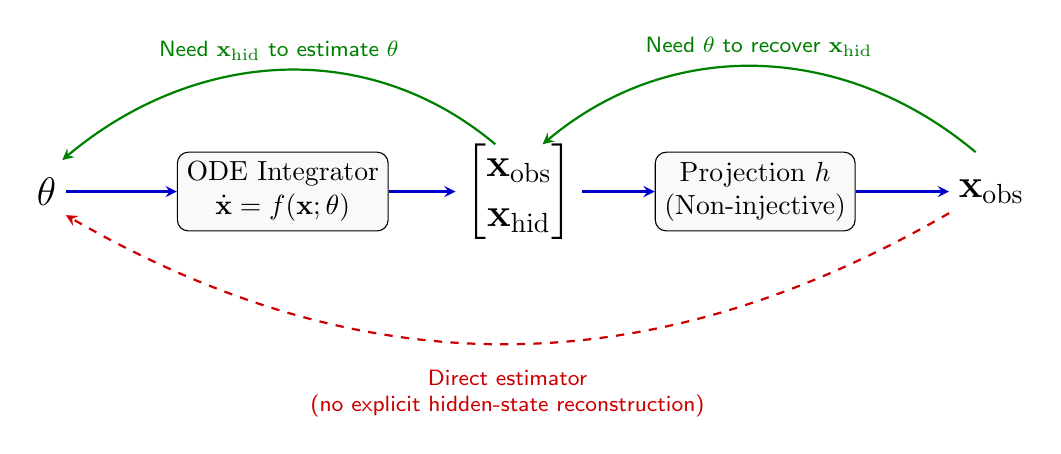
\begin{tikzpicture}[
    >=stealth,
    box/.style={draw, rectangle, rounded corners, minimum width=2.2cm, minimum height=1.0cm, align=center, fill=gray!5},
    fwd_arrow/.style={->, thick, blue!80!black},
    inv_arrow/.style={->, thick, dashed, red!80!black},
    step_arrow/.style={->, thick, green!50!black},
    label_font/.style={font=\footnotesize\sffamily, align=center} % align=center 추가하여 줄바꿈 가능하게 함
]

% 1. 노드 간격을 좁혀서 밀도(Compactness) 확보
\node (theta) at (0, 0) {\Large $\theta$};
\node[box] (ode) at (3.0, 0) {ODE Integrator \\ $\dot{\mathbf{x}} = f(\mathbf{x}; \theta)$};
\node (full_x) at (6.0, 0) {\Large $\begin{bmatrix} \mathbf{x}_{\mathrm{obs}} \\ \mathbf{x}_{\mathrm{hid}} \end{bmatrix}$};
\node[box] (proj) at (9.0, 0) {Projection $h$ \\ (Non-injective)};
\node (x_obs) at (12.0, 0) {\Large $\mathbf{x}_{\mathrm{obs}}$};

% 2. Forward Process (파란색)
\draw[fwd_arrow] (theta) -- (ode);
\draw[fwd_arrow] (ode) -- (full_x);
\draw[fwd_arrow] (full_x) -- (proj);
\draw[fwd_arrow] (proj) -- (x_obs);

% 3. Naive Direct Mapping (빨간색 점선)
% 화살표가 겹치지 않도록 시작점(south west)과 도착점(south east) 지정, 텍스트 두 줄 처리
\draw[inv_arrow] (x_obs.south west) to[out=-150, in=-30]
    node[below, label_font, text=red!80!black, yshift=-2mm] {Direct estimator \\ (no explicit hidden-state reconstruction)}
    (theta.south east);

% 4. Step-by-step Inversion (초록색 딜레마)
% 포물선 곡률을 넉넉하게 주어 박스와 겹치지 않게 함
\draw[step_arrow] (11.8, 0.5) to[out=140, in=40] 
    node[above, label_font, text=green!50!black] {Need $\theta$ to recover $\mathbf{x}_{\mathrm{hid}}$} 
    (6.3, 0.6);
    
\draw[step_arrow] (5.7, 0.6) to[out=140, in=40] 
    node[above, label_font, text=green!50!black] {Need $\mathbf{x}_{\mathrm{hid}}$ to estimate $\theta$} 
    (0.2, 0.4);

\end{tikzpicture}
\end{document}